\documentclass[12pt]{article} % размер шрифта

\usepackage{tikz} % картинки в tikz
\usepackage{microtype} % свешивание пунктуации

\usepackage{array} % для столбцов фиксированной ширины
\usepackage{url} % для вставки ссылок \url{...}

\usepackage{indentfirst} % отступ в первом параграфе

\usepackage{sectsty} % для центрирования названий частей
\allsectionsfont{\centering} % приказываем центрировать все sections

\usepackage{amsthm} % теоремы и доказательства
\usepackage{mathtools}


\theoremstyle{definition} % прямой шрифт в условии теорем
\newtheorem{theorem}{Теорема}[section]
\newtheorem{exercise}{Упражнение}[section]


\usepackage{amsmath, amssymb} % куча стандартных математических плюшек
\usepackage[top=2cm, left=1.5cm, right=1.5cm, bottom=2cm]{geometry} % размер текста на странице

\usepackage{lastpage} % чтобы узнать номер последней страницы

\usepackage{enumitem} % дополнительные плюшки для списков
%  например \begin{enumerate}[resume] позволяет продолжить нумерацию в новом списке
\usepackage{caption} % подписи к картинкам без плавающего окружения figure

\usepackage{hyperref} % гиперссылки

\usepackage{verbatim} % побуквенный вывод

\usepackage{fancyhdr} % весёлые колонтитулы
\pagestyle{fancy}
\lhead{Эконометрика, финтех}
\chead{}
\rhead{2018-12-11, встреча 10}
\lfoot{}
\cfoot{}
\rfoot{\thepage/\pageref{LastPage}}
\renewcommand{\headrulewidth}{0.4pt}
\renewcommand{\footrulewidth}{0.4pt}



\usepackage{todonotes} % для вставки в документ заметок о том, что осталось сделать
% \todo{Здесь надо коэффициенты исправить}
% \missingfigure{Здесь будет картина Последний день Помпеи}
% команда \listoftodos — печатает все поставленные \todo'шки

\usepackage{booktabs} % красивые таблицы
% заповеди из документации:
% 1. Не используйте вертикальные линии
% 2. Не используйте двойные линии
% 3. Единицы измерения помещайте в шапку таблицы
% 4. Не сокращайте .1 вместо 0.1
% 5. Повторяющееся значение повторяйте, а не говорите "то же"

\usepackage{fontspec} % поддержка разных шрифтов
\usepackage{polyglossia} % поддержка разных языков

\setmainlanguage{russian}
\setotherlanguages{english}

\setmainfont{Linux Libertine O} % выбираем шрифт
% если Linux Libertine не установлен, то
% можно также попробовать Helvetica, Arial, Cambria и т.Д.

% чтобы использовать шрифт Linux Libertine на личном компе,
% его надо предварительно скачать по ссылке
% http://www.linuxlibertine.org/index.php?id=91&L=1

% на сервисах типа sharelatex.com этот шрифт есть :)

\newfontfamily{\cyrillicfonttt}{Linux Libertine O}
% пояснение зачем нужно шаманство с \newfontfamily
% http://tex.stackexchange.com/questions/91507/

\AddEnumerateCounter{\asbuk}{\russian@alph}{щ} % для списков с русскими буквами
%\setlist[enumerate, 2]{label=\asbuk*),ref=\asbuk*} % списки уровня 2 будут буквами а) б) ...

%% эконометрические и вероятностные сокращения
\DeclareMathOperator{\Cov}{Cov}
\DeclareMathOperator{\sCov}{sCov}
\DeclareMathOperator{\sVar}{sVar}
\DeclareMathOperator{\sCorr}{sCorr}
\DeclareMathOperator{\Corr}{Corr}
\DeclareMathOperator{\Var}{Var}
\DeclareMathOperator{\E}{E}
\DeclareMathOperator{\tr}{trace}
\DeclareMathOperator{\trace}{trace}
\DeclareMathOperator{\plim}{plim}

\def \hb{\hat{\beta}}
\def \hs{\hat{\sigma}}
\def \htheta{\hat{\theta}}
\def \s{\sigma}
\def \hy{\hat{y}}
\def \hY{\hat{Y}}
\def \v1{\vec{1}}
\def \e{\varepsilon}
\def \he{\hat{\e}}
\def \z{z}
\def \hVar{\widehat{\Var}}
\def \hCorr{\widehat{\Corr}}
\def \hCov{\widehat{\Cov}}
\def \cN{\mathcal{N}}
\def \RR{\mathbb{R}}


\begin{document}
Конспектировала: Света Жучкова.

\section{Блочные матрицы}
Если размеры блоков допускают операцию умножения, то:

\[
\left[
\begin{array}{c|c}
A & B \\
\hline
C & D
\end{array}
\right]
\cdot
\left[
\begin{array}{c|c}
E & F \\
\hline
G & H
\end{array}
\right]
=
\left[
\begin{array}{c|c}
AE + BG &  \ldots\\
\hline
\ldots & \ldots
\end{array}
\right]
\]

\begin{exercise}
Блочное обращение.
\[
\begin{bmatrix}
A & B \\
0 & C
\end{bmatrix}^{-1}
= \\
?
\]

Предположения: $
\det A_{n \times n} \neq 0; \quad \det C_{k \times k} \neq 0$.

Способы решения:
\begin{enumerate}
\item Интуиция.

Если бы матрицы были числами:

\[ \displaystyle
\begin{pmatrix} a & b\\ 0 & c \end{pmatrix}^{-1} = \frac{1}{ac} \begin{pmatrix} c & -b\\ 0 & a \end{pmatrix} = \begin{pmatrix} \frac{1}{a} & \frac{-b}{ac} \\ 0 & \frac{1}{c} \end{pmatrix} = \begin{pmatrix} A^{-1}_{n \times n} & -BA^{-1}C^{-1}_{n \times k} \\ 0 & C^{-1}_{k \times k} \end{pmatrix}
\]

\item Метод Гаусса.
\[
\left[
\begin{array}{c|c}
A_{n \times n} \quad B_{n \times k} & I \quad 0 \\
0 \quad \quad \quad C_{k \times k} & 0 \quad I
\end{array}
\right] \Rightarrow
\left[
\begin{array}{l|c}
I \quad A^{-1}B & A^{-1} \quad 0 \\
0 \quad \quad C & 0 \quad \quad I
\end{array}
\right] \Rightarrow
\left[
\begin{array}{l|c}
I \quad A^{-1}B & A^{-1} \quad 0 \\
0 \quad \quad I & 0 \quad C^{-1}
\end{array}
\right] \Rightarrow
\]
\[
\Rightarrow
\left[
\begin{array}{c|l}
I \quad 0 & A^{-1} \quad -A^{-1}BC^{-1} \\
0 \quad I & 0 \quad \quad \quad \quad C^{-1}
\end{array}
\right]
\]


\item Система уравнений.
\[
\begin{pmatrix} A & B \\ 0 & C \end{pmatrix} \cdot \begin{pmatrix} X & Y \\ Z & W \end{pmatrix} = \begin{pmatrix} I & 0 \\ 0 & I \end{pmatrix}
\]
\renewcommand{\labelenumii}{\arabic{enumii}.}
\begin{enumerate}
    \item $0X + CZ = 0 \Rightarrow Z = 0$
    \item $AX + BZ = I  \Rightarrow X = A^{-1}$
    \item \dots
\end{enumerate}

\end{enumerate}

\end{exercise}

\textbf{Утверждение.}
Если выполняются предпоссылки теоремы Гаусса-Маркова и $u_i \sim \mathcal{N}(0, \sigma^2)$, то

\[ \frac{\hat{\beta}_j - \beta_j}{se(\hat{\beta}_j)} \sim t_{n-k},
\]

\[\frac{(RSS_{R} - RSS_{UR})/(k_{UR} - k_{R})}{RSS_{UR}/(n - k_{UR})} \sim F_{(k_{UR} - k_{R})(n - k_{UR})}.
\]

И этими статистиками можно проверять одни и те же гипотезы! Например, $H_0: \beta_{7} = 0$.


\textbf{Утверждение.} Если \ldots
\begin{enumerate}
    \item Выполняются предпоссылки теоремы Гаусса-Маркова;
    \item $u_i \sim \mathcal{N}(0, \sigma^2)$;
    \item Оцениваются две модели:

    Неограниченная (UR): $\hat{y} = X\beta$,

    Ограниченная (R): $\hat{y} = X\beta$ при $\beta_j = 0$;
    \item Проверяется гипотеза $H_{0}: \hat{\beta_j} = 0$
\end{enumerate}

\begin{center}
\ldots то  $t^2 = F$.
\end{center}

\textbf{Доказательство} (для $\hat{\beta_1}$ при условии, что все регрессоры центрированы):
\[ \hat{\Var}(\hb{}) = \frac{RSS}{n - k} \cdot (X^{T} X)^{-1}
\]
\[ \hat{\beta} = (X^{T} X)^{-1} X^{T}y = \begin{bmatrix}
           \hb{}_{1} \\
           \hb{}_{2} \\
           \vdots \\
           \hb{}_{n}
         \end{bmatrix}
\]
\[ t_1 = \frac{\hat{\beta_1}}{\sqrt{\frac{RSS}{n - k} (X^T X)^{-1}_{[1, 1]}}}
\]
\[ t^2_1 = \frac{\hat{\beta_1}^2}{\frac{RSS}{n - k} (X^T X)^{-1}_{[1, 1]}}
\]

Часть в знаменателе $\displaystyle \frac{RSS}{n - k}$ нашли. Тогда осталось сравнить:
\[
\frac{\hat{\beta_1}^2}{(X^T X)^{-1}_{[1, 1]}} \quad vs \quad (RSS_{R} - RSS_{UR}),
\]

так как $k_{UR} - k_{R} = 1$ (проверяем гипотезу об одном коэффициенте).

Поскольку по условию все переменные центрированы:

\[ (X^T X)^{-1}_{[1, 1]} = \frac{1}{RSS_{1}},\]

где $RSS_1$ -- $RSS$ в регрессии первого столбца $X$ на остальные.
То есть осталось сравнить:
\[
\hat{\beta_1}^2 \cdot RSS_1 \quad vs \quad (RSS_{R} - RSS_{UR})
\]

Докажем геометрически, воспользовавшись иллюстрацией.

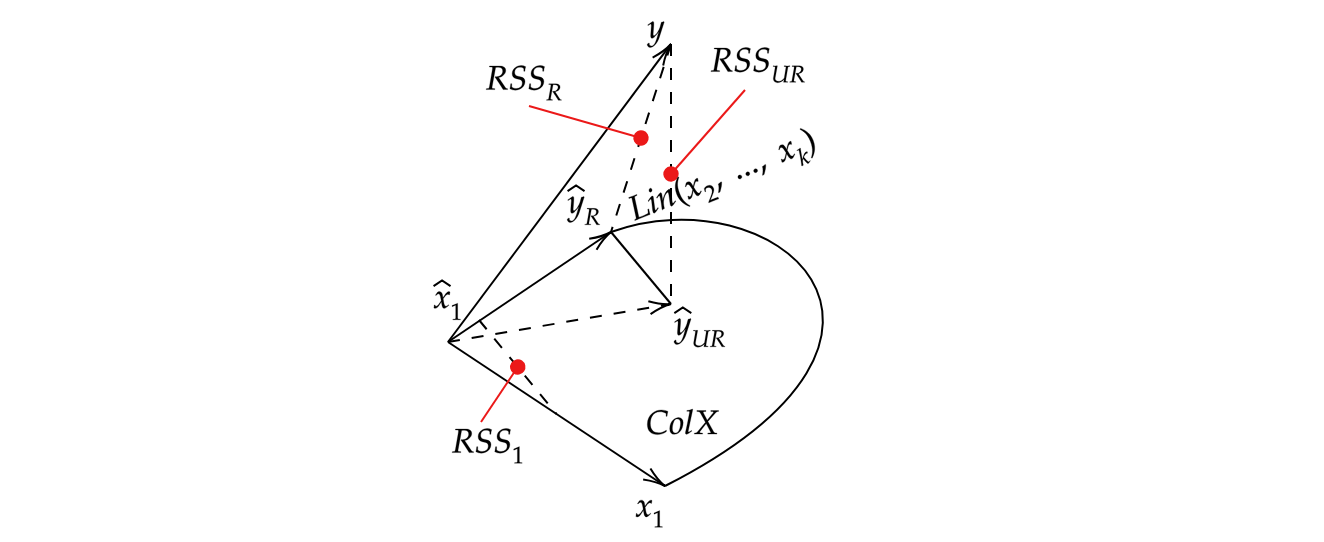
\includegraphics[width=0.8\linewidth]{images/10_picture1.png}

По теореме о трёх перпендикулярах:

\[ (\hat{y}_{UR} - \hat{y}_{R}) \perp Lin(x_2, \ldots, x_n),
\]
\[
(x_1 -\hat{x_1}) \perp Lin(x_2, \ldots, x_n),
\]
\[\hat{y}_{UR} - \hat{y}_{R}, x_1 - \hat{x_1} \in Col X,\]
\[\dim Col X = k = \dim Lin(x_2, \ldots, x_n) \neq 1 \Rightarrow x_1 - \hat{x_1} \parallel \hat{y}_{UR} - \hat{y}_{R}.\]

Введём обозначение $\tilde{y}_{UR}$:
\[ \hy{}^{UR} = X \hb{}^{UR}
\]
\[ \hy{}^{UR} = \hb{}_1^{UR} x_1 + \hb{}_2^{UR} x_2 + \dots + \hb{}_k^{UR} x_k
\]
\[ \tilde{y}_{UR} = \hb{}_2^{UR} x_2 + \dots + \hb{}_k^{UR} x_k
\]

Рассмотрим этот рисунок подробнее, разложив проекцию по базису и обозначив все интересующие нас треугольники.

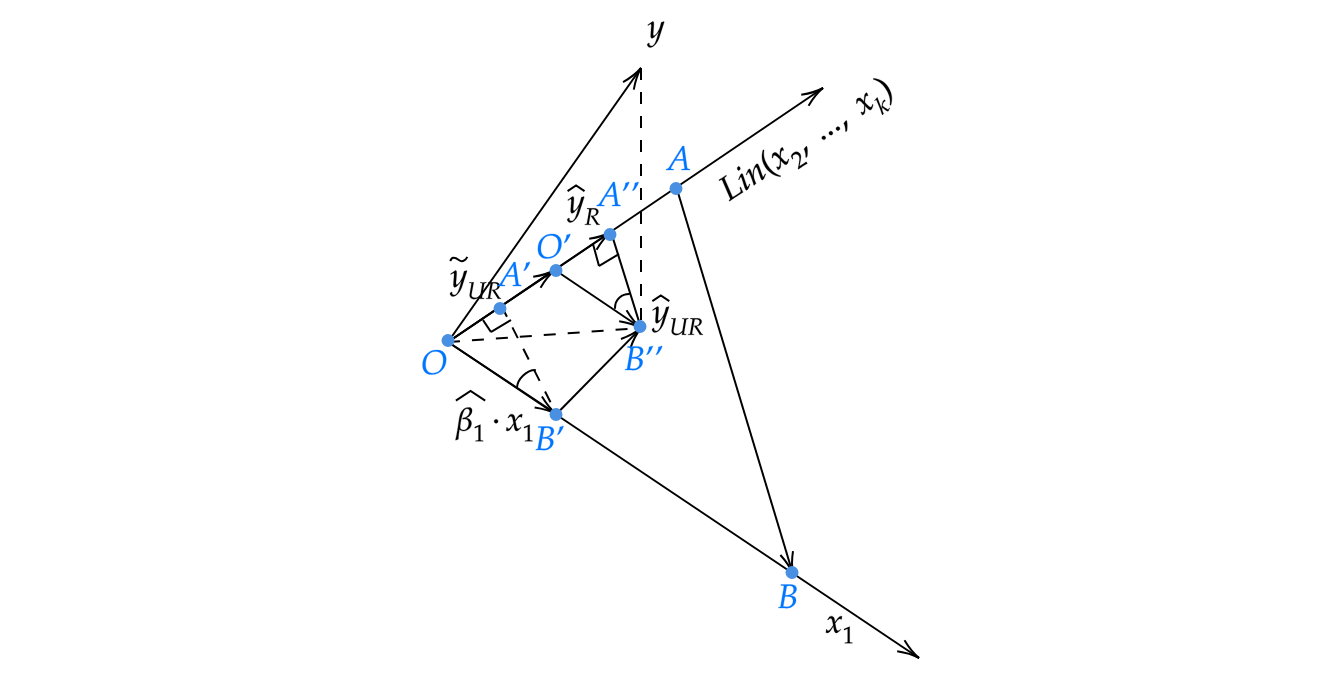
\includegraphics[width=0.8\linewidth]{images/10_picture2.png}


Итак, нужно сравнить:
\[ \hb{}_1^2 \cdot (AB)^2 \quad vs \quad  (A''B'')^2
\]

\begin{enumerate}
    \item $|A'B'| = |\hb{}_1|\cdot |AB| \Rightarrow  (A'B')^2 \quad vs \quad (A''B'')^2
    $
    \item

    $\begin{rcases}
    \Delta OAB \sim \Delta OA'B' \\
    \Delta OA'B' = \Delta O'A''B''
    \end{rcases}
    \text{$\Rightarrow (A'B')^2 = (A''B'')^2$}$
\end{enumerate}





\section{Состоятельность МНК-оценок}

Пусть дана последовательность случайных величин $z_1, z_2, \ldots, z_n$. Пределом по вероятности называют величину $\plim_{n\to\infty}{z_n} = w$ или $z_n \xrightarrow{p} w$.

\textbf{Определение.} $\lim_{n\to\infty}{p(|z_n - w| > \epsilon)}=0$ для любого $\epsilon > 0$.

Как рассчитывать предел по вероятности:
\begin{enumerate}
\item Используя свойства обычных пределов;

\item Используя закон больших чисел (ЗБЧ): если $z_1, z_2, \ldots, z_n$ независимы и одинаково распределены, то $\displaystyle \plim_{n\to\infty}{\bar{z_n}}=\mathbb{E}(z_1)$;

\item Используя неравенство Чебышёва: если $\mathbb{E}(z_n)\to\mu$, т.е. $\lim{\mathbb{E}(z_n)}=0$ и $\lim{\Var(z_n)}=0$, то $\displaystyle \plim\limits_{n\to\infty}{z_n}=\mu$.
\end{enumerate}

\begin{exercise}
Пары $(z_i, w_i)$ одинаково распределены и независимы, т.е. сами $z_i, w_i$ могут быть зависимы, но $z_1, \ldots, z_n$ независимы и $w_1, \ldots, w_n$ независимы. Найти предел по вероятности:
\[\plim\limits_{n\to\infty} \frac{\sum{(z_i-\bar{z})\cdot(w_i-\bar{w})}}{n-1} = \\
?\]

Решение.
\[
\plim\limits_{n\to\infty} \frac{\sum{(z_i-\bar{z})\cdot(w_i-\bar{w})}}{n-1} =
\]
\[=
\plim\limits_{n\to\infty}\frac{\sum{z_i w_i}}{n-1} - \plim\limits_{n\to\infty}\frac{\bar{z}\sum{w_i}}{n-1} - \plim\limits_{n\to\infty}\frac{\bar{w}\sum{z_i}}{n-1} - \plim\limits_{n\to\infty}\frac{n\bar{z}\bar{w}}{n-1}
=
\]
\[=
\mathbb{E}(z_1, w_1) - \mathbb{E}(z_1)\cdot\mathbb{E}(w_1) - \mathbb{E}(w_1)\cdot\mathbb{E}(z_1) - \mathbb{E}(w_1)\cdot\mathbb{E}(z_1) =
\]
\[=
\mathbb{E}(z_1, w_1) - \mathbb{E}(z_1)\cdot\mathbb{E}(w_1) = \Cov(z_1, w_1).
\]


\end{exercise}

\begin{exercise}
Пусть есть следующая зависимость:
\[ y_i = \beta_1 + \beta_2 \cdot x_i + u_i,
\]
где $x_i$ -- количество съеденных студентом за семестр конфет, $y_i$ -- его оценка за курс по эконометрике. Настоящие $y_i$ и $x_i$ неизвестны, зато известна $x_i^*$:
\[
x_i^* = x_i + \alpha + \nu_i,
\]
где $\alpha$ -- это константа, обозначающая национальную русскую скромность, $\alpha < 0$; $\nu_i$ -- ошибка воспоминаний.

$x_i, \nu_i,  u_i$ независимы.

$\mathbb{E}(x_i) = \mu_x$; $\mathbb{E}(u_i) = \mathbb{E}(\nu_i) = 0$.

$\Var(x_i) = \sigma_x^2$;
$\Var(u_i) = \sigma_u^2$;
$\Var(\nu_i) = \sigma_{\nu}^2$.

Построим регрессию и определим, будет ли оценка $\hat{\beta_2}$ состоятельной:
\[
\hat{y_i} = \hat{\beta_1} + \hat{\beta_2} \cdot x_i^*.
\]

Решение.

\[
\plim\limits_{n\to\infty}\hat{\beta_2} = \plim\limits_{n\to\infty}\frac{\sum{(x_i^* - \bar{x^*)}(y_i - y)/(n - 1)}}{\sum{(x_i^* - \bar{x^*})^2}/(n-1)}=
\]
\[=
\frac{\Cov(x_i^*, y_i)}{\Var(x_i^*)} = \frac{\Cov(x_i + \alpha +\nu_i, \beta_1 + \beta_2 \cdot x_i + u_i)}{\sigma_x^2 + \sigma_\nu^2} = \frac{\beta_2 \cdot \sigma_x^2}{\sigma_x^2 \cdot \sigma_\nu^2} \neq \beta_2,
\]
\[
0 < \frac{\sigma_x^2}{\sigma_x^2 \cdot \sigma_\nu^2} < 1.
\]

Вывод: оценка не состоятельна!
\end{exercise}


\begin{exercise}
Винни-Пух и Пятачок ходили в гости к Кролику. После нескольких визитов друзья решили оценить зависимость:

\[ y_i = \beta_1 + \beta_2 \cdot x_i + u_i,
\]
где $x_i$ -- количество горшков, $y_i$ -- количество времени, потраченное Винни-Пухом на то, чтобы выбраться из норы Кролика.

Пятачок записывал свои наблюдения:
$x_i^n = x_i + \nu_i$.

И Кролик записывал свои наблюдения:
$x_i^k = x_i + \eta_i$.

Наблюдения независимы и одинаково распределены.

$x_i, \nu_i, \eta_i,  u_i$ также независимы.

$\mathbb{E}(x_i) = \mu_x$; $\mathbb{E}(u_i) = \mathbb{E}(\nu_i) = \mathbb{E}(\eta_i) = 0$.

$\Var(x_i) = \sigma_x^2$;
$\Var(u_i) = \sigma_u^2$;
$\Var(\nu_i) = \sigma_{\nu}^2$;
$\Var(\eta_i) = \sigma_{\eta}^2$.

Пятачок попытался построить регрессию:
\[
\hat{y}_i = \hat{\beta}_1^n + \hat{\beta}_2^n \cdot x_i^n.
\]

\begin{enumerate}
    \item

    Состоятельная ли оценка Пятачка? Найдём соответствующий предел по вероятности, аналогичный пределу в предыдущем задании:

    \[\displaystyle \plim_{n \rightarrow \infty} \hat{\beta}_n^2 = \beta_2 \cdot \frac{\sigma_x^2}{\sigma_x^2 + \sigma_{\nu}^2}.\]

    \item Найдём ещё предел по вероятности:
    \[\displaystyle \plim_{n \rightarrow \infty} \frac{\sum (x_i^n - \bar{x}^n)(x_i^k - \bar{x}^k)}{n - 1} = \Cov(x_1^n, x_1^k) = \sigma_x^2.\]

    \item Как скорректировать оценку, чтобы она стала состоятельна? Настоящая $\sigma_x^2$ неизвестна.
\end{enumerate}



Рассмотрим варианты и для оценки Пятачка, и для оценки Кролика:
\begin{enumerate}
    \item $\displaystyle \hat{\beta}_{2}^n$ (скорр.) = $\displaystyle \hat{\beta}_{2}^n \cdot \frac{\sum (x_i^n - \bar{x}^n)}{\underbrace{\sum (x_i^n - \bar{x}^n)(x_i^k - \bar{x}^k)}_\text{коэффициент в регрессии $x_i^k$ на $x_i^n$}} = \frac{\hat{\beta}_{2}^n}{\hat{\gamma_2}} = \frac{\sum (x_i^n - \bar{x}^n)(y_i - \bar{y})}{\sum (x_i^n - \bar{x}^n)(x_i^k - \bar{x}^k)}$.

    Откуда взять $\hat{\gamma_2}$? Из соответствующей регрессии: $\hat{x}_i^k = \hat{\gamma}_i + \hat{\gamma}_2 \cdot x_i^{n}$.

    \item Аналогично корректируется и оценка Кролика: $\displaystyle \hat{\beta}_{2}^k$ (скорр.) = $\displaystyle \frac{\sum (x_i^k - \bar{x}^k)(y_i - \bar{y})}{\sum (x_i^n - \bar{x}^n)(x_i^k - \bar{x}^k)}$.
\end{enumerate}

\end{exercise}

\begin{exercise}
Пусть дана зависимость $y_i = \beta_1 + \beta_2 x_i + u_i$,

где $x_i=\begin{cases}
               \displaystyle 0, i = 1, \\
               \displaystyle 1, i > 1. \\
            \end{cases}$


$\mathbb{E}(u_i) = 0$, $\Var(u_i) = \sigma^2$.

$\Cov(u_i, u_j) = 0$ при $i \neq j$.

Теорема Гаусса-Маркова соблюдена. Будет ли состоятельной оценка $\hat{\beta}_2$?

\theoremstyle{definition}{Решение.}

\[ \displaystyle \bar{x} = \frac{n - 1}{n} \]

\[ \displaystyle \sum (x_i - \bar{x})^2 = (n - 1) \cdot (1 - \frac{n - 1}{n})^2 + (\frac{n - 1}{n})^2 = \frac{n - 1}{n^2} + \frac{(n - 1)^2}{n^2} = \frac{n(n - 1)}{n^2} = \frac{n - 1}{n} \xrightarrow[n \to \infty]{} 1 \]

\[ \displaystyle \hat{\beta}_2 = \frac{\sum (y_i - \bar{y})(x_i - \bar{x})}{\sum (x_i - \bar{x})^2} = \]
\[ = \frac{\sum y_i (x_i - \bar{x}) - \overbrace{\bar{y}\sum(x_i - \bar{x})}^{=0}}{\sum (x_i - \bar{x})^2} = \frac{\beta_1 \overbrace{\sum (x_i - \bar{x})}^{=0} + \beta_2 \sum x_i (x_i - \bar{x}) + \sum u_i (x_i - \bar{x})}{\sum (x_i - \bar{x})^2} = \]

\[
= \displaystyle  \frac{\beta_2 \sum (x_i - \bar{x})^2}{\sum (x_i - \bar{x})^2} + \frac{\sum u_i (x_i - \bar{x})}{\sum (x_i - \bar{x})^2} = \beta_2 + \frac{\sum u_i (x_i - \bar{x})}{\sum (x_i - \bar{x})^2} =
\beta_2 + \frac{u_1(x_1 - \bar{x}) + \sum_{i=2}^n u_i(x_i - \bar{x})}{\sum (x_i - \bar{x})^2} = \]

\[
= \displaystyle \beta_2 + \frac{-u_1 \bar{x} + (1 - \bar{x})\sum_{i=2}^n u_i}{\sum (x_i - \bar{x})^2} = \beta_2 + \frac{-u_1 \frac{n - 1}{n} + (1 - \frac{n - 1}{n})\sum_{i=2}^n u_i }{\frac{n - 1}{n}} = \beta_2 - u_1 + \frac{1}{n - 1} \sum_{i=2}^n u_i
.\]

\[ \plim \hat{\beta}_2 = \plim (\beta_2 - u_1 + \frac{1}{n - 1} \overbrace{\sum_{i=2}^n u_i)}^\text{ЗБЧ: $\mathbb{E}(u_2)$} = \beta_2 - u_1 + \overbrace{\mathbb{E}(u_2)}^{=0} = \beta_2 - u_1
.\]

Вывод: оценка не состоятельна!
\end{exercise}
\end{document}
